\documentclass{article}
\usepackage{graphicx}
\usepackage{amsmath}
\usepackage{hyperref}
\usepackage{pgfplots}
\title{Bio Signal Amplifier}
\author{Abhishek Amit Raje}
\date{November 2023}

\hypersetup{
    colorlinks=true,
    linkcolor=red,
    urlcolor=red
}
\begin{titlepage}
  \centering
  
\includegraphics[width=0.4\textwidth]{iithlogo.png}\par\vspace{1cm}
  {\scshape\LARGE Indian Institute of Technology Hyderabad \par}
  \vspace{1cm}
  {\scshape\Large Analog Electronics and Integrated Circuits \par}
  \vspace{1.5cm}
  \maketitle
\end{titlepage}
\begin{document}

\maketitle

\section{Circuit Design for ECG}

The approach taken to build the instrumentation amplifier is to use two buffer circuits for the two terminals of the ECG and one difference amplifier.

\begin{figure}[h]
  \centering
  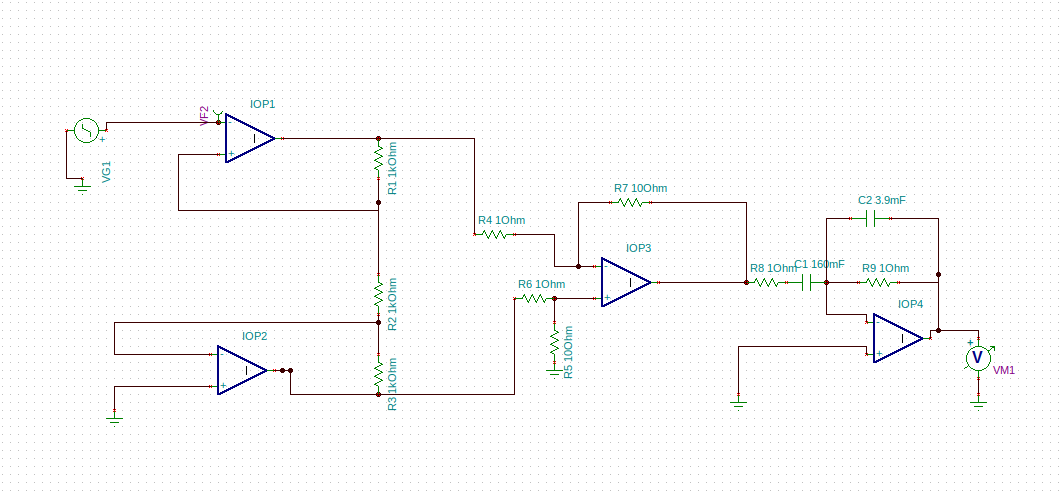
\includegraphics[width=1\textwidth]{ECG_Circuit.png} 
  \caption{Circuit diagram for ECG signal amplification.}
  \label{fig:ecg-circuit}
\end{figure}

\section{Instrumentation Amplifier Analysis}
For any general \(R_1\), \(R_2\), \(R_3\), \(R_4\) of the operational amplifier, the total amplification is given by:
\[
\frac{V_0}{V_1 - V_2} = \frac{R_4}{R_3} \left(1 + 2 \frac{R_1}{R_2}\right)
\]

\begin{figure}[h]
  \centering
  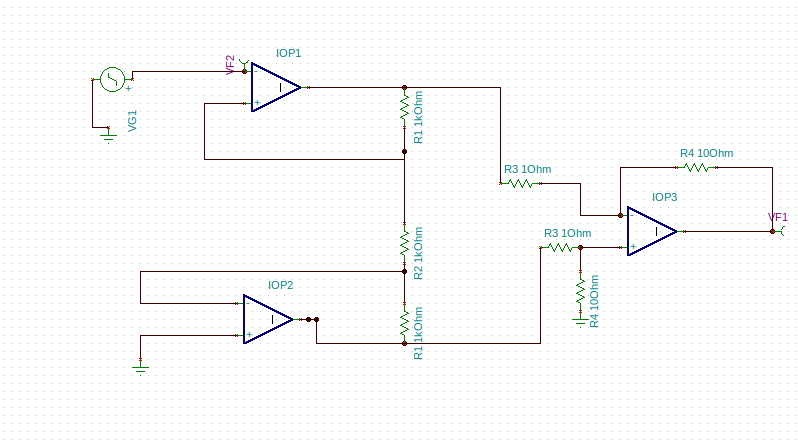
\includegraphics[width=0.8\textwidth]{Instrumentation.png} 
  \caption{Instrumentation Amplifier Design.}
  \label{fig:instrumentation-amp}
\end{figure}
\begin{figure}[h]
  \centering
  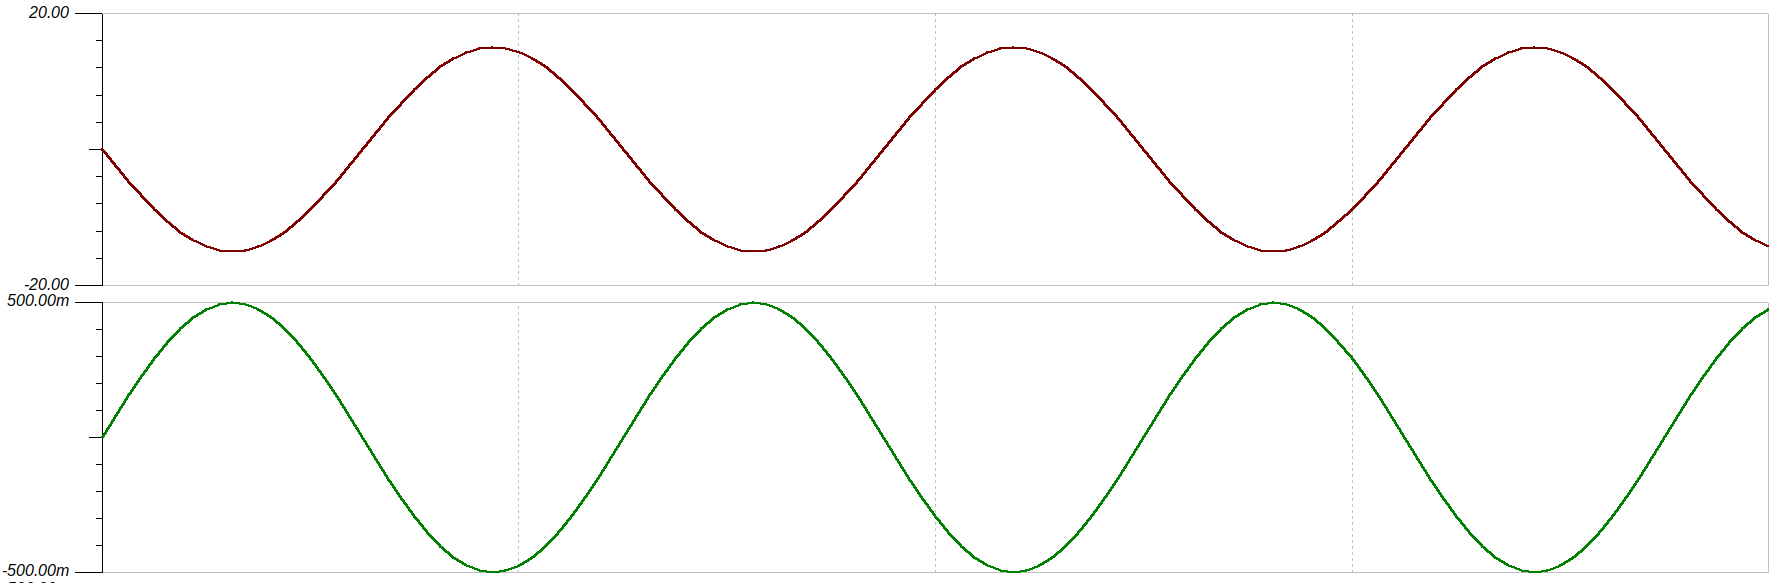
\includegraphics[width=1\textwidth]{sinamp.png} 
  \caption{Input Output Characteristics of ECG Amplifier for a general sine wave}
  \label{fig:instrumentation-amp}
\end{figure}

\begin{figure}[h]
  \centering
  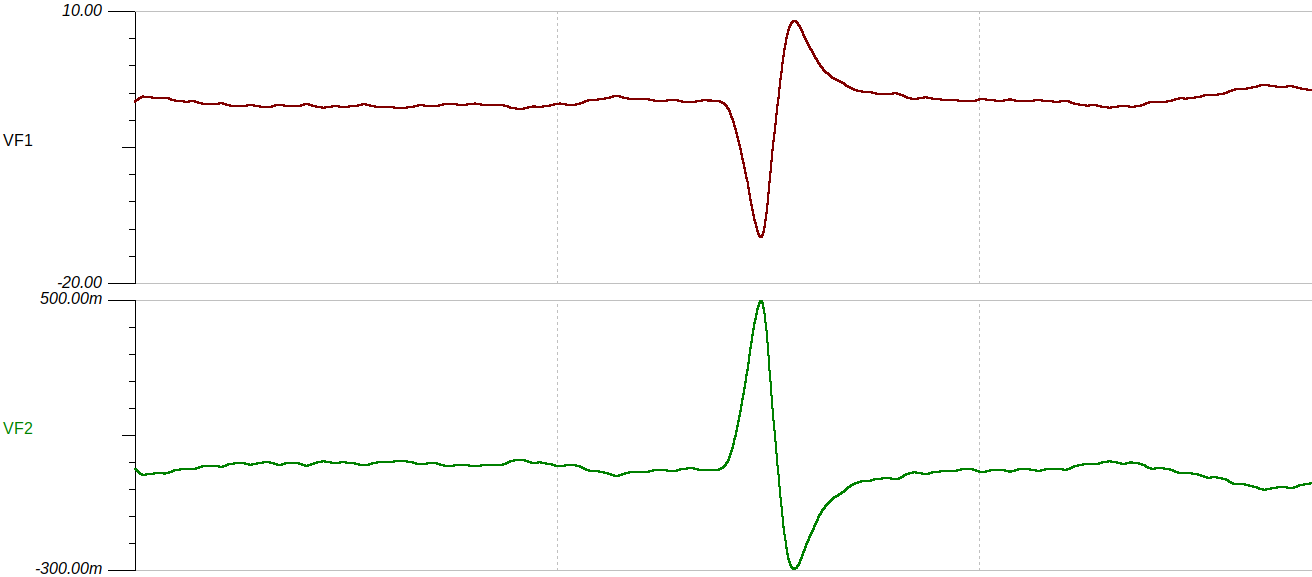
\includegraphics[width=1\textwidth]{Input_Output_ECG.png} 
  \caption{Input Output Characteristics of ECG Amplifier for ecg signal}
  \label{fig:instrumentation-amp}
\end{figure}
The input signal has been taken from a .wav file
\newpage
\section{Amplification Analysis}
\textbf{Proof:}

Amplification due to buffer
\begin{align*}
v^- &= v^+ \\
v_1^+ & = V_{\text{signal}} \\
v_2^+ & = 0 \\
i_d & = \frac{V_{\text{signal}}}{R_2} \\
V_{o1} & = V_{\text{signal}}\left(1 + \frac{R_1}{R_2}\right) \\
V_{o2} & = V_{\text{signal}}\left(-\frac{R_1}{R_2}\right)
\end{align*}
Amplification due to difference amplifier
\[
-\frac{R_4}{R_3}(V_{o1} - V_{o2})
\]

Therefore, the net amplification is given by
\[
\text{Amplification} = \frac{R_4}{R_3} \left(1 + 2 \frac{R_1}{R_2}\right)
\]
\begin{align*}
& \text{Signal being amplified: ECG (5mV)} \\
& R_1 = R_2 = 1 \, \text{k}\Omega \\
& R_4 = 1000R_3 \\
& \text{Net Gain} = 3000
\end{align*}

Note: \(R_4/R_3 = 10\) (as the .wav file has an amplitude of 500mV)
\newpage
\section{Filter Analysis}
\begin{figure}[h]
  \centering
  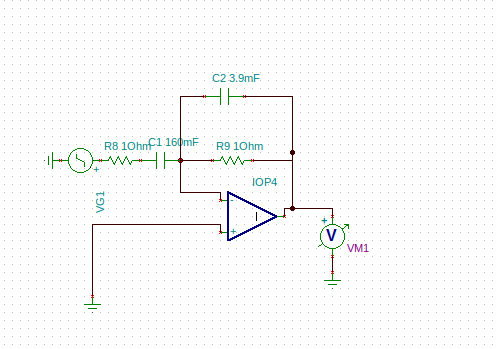
\includegraphics[width=0.9\textwidth]{Filter.png} 
  \caption{Filter Design}
  \label{fig:instrumentation-amp}
\end{figure}
\begin{figure}[h]
  \centering
  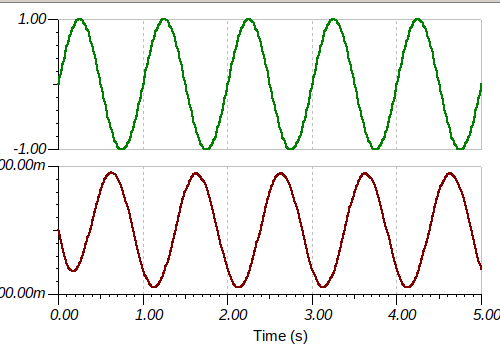
\includegraphics[width=0.5\textwidth]{1hz.png} 
  \caption{Input Output Characteristics at f=1Hz}
  \label{fig:instrumentation-amp}
\end{figure}

\begin{figure}[h]
  \centering
  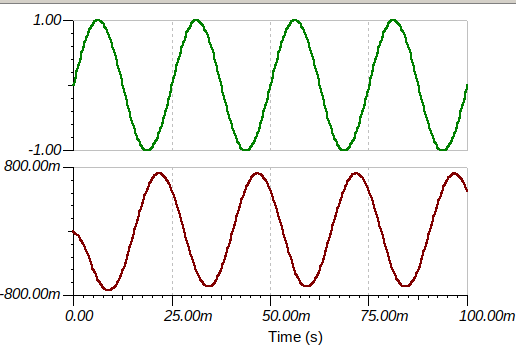
\includegraphics[width=0.7\textwidth]{40Hz.png} 
  \caption{Input Output Characteristics at f=40Hz}
  \label{fig:instrumentation-amp}
\end{figure}

\begin{figure}[h]
  \centering
  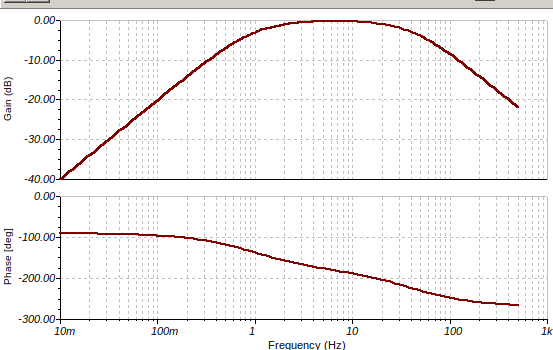
\includegraphics[width=0.7\textwidth]{BodePlot.png} 
  \caption{Bode Plot of the Filter Circuit}
  \label{fig:instrumentation-amp}
\end{figure}
\newpage
The circuit is designed such that
\[
f_0 = \frac{1}{2\pi \sqrt{R_1 R_2 C_1 C_2}}
\]
For the given values:
\[
f_0 = 6.32 \, \text{Hz}
\quad
f_l = 1 \, \text{Hz}
\quad
f_h = 40 \, \text{Hz}
\]
As depicted 1Hz and 40 Hz are the half power frequencies where the output wave is 0.707 times the input wave
\section{Transfer Function}
\[
v_{\text{in}} - iR_1 - \frac{i}{C_1s} - \frac{i}{C_2s(1 + C_2s)} = V_0
\]

\[
i = \frac{v_{\text{in}}}{R_1+ \frac{1}{c_1s}} 
\]
on solving we get 
\[
H(s) = -\frac{c_1}{c_2} \cdot \frac{1}{(R_1C_1s + 1)(R_2C_2s + 1)}
\]
This equation describes the relationship between the input (\( v_{\text{in}} \)) and output (\( V_0 \)) signals in the High Pass filter circuit.

\begin{figure}[h]
  \centering
  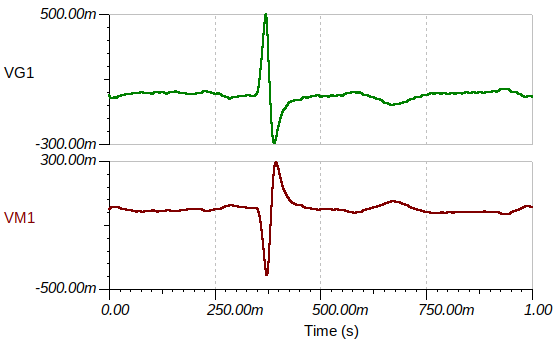
\includegraphics[width=0.9\textwidth]{ECG_Filter.png} 
  \caption{ECG signal before and after filtering}
  \label{fig:instrumentation-amp}
\end{figure}
\newpage
\section{Final Implementation}
\begin{figure}[h]
  \centering
  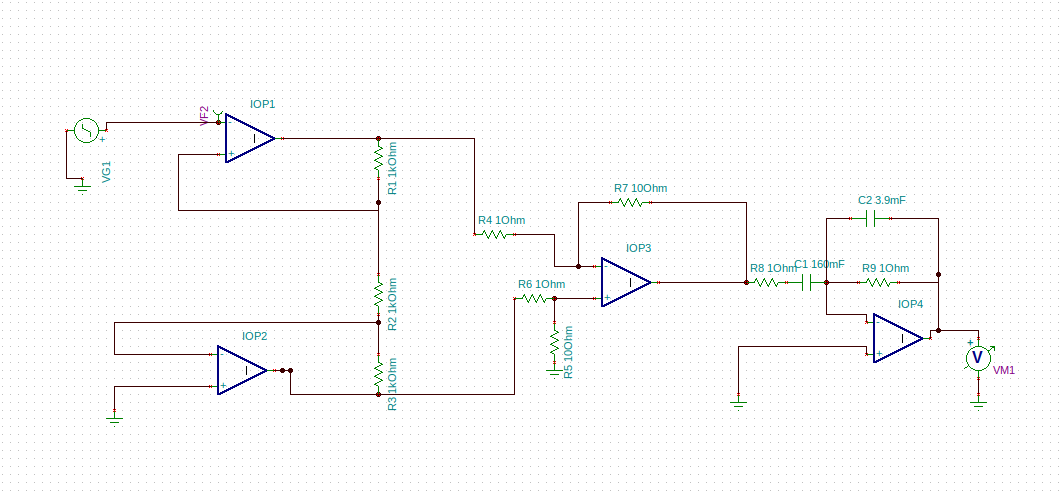
\includegraphics[width=0.9\textwidth]{ECG_Circuit.png} 
  \caption{Circuit including Instrumentation Amplifier and Filter}
  \label{fig:instrumentation-amp}
\end{figure}

\begin{figure}[h]
  \centering
  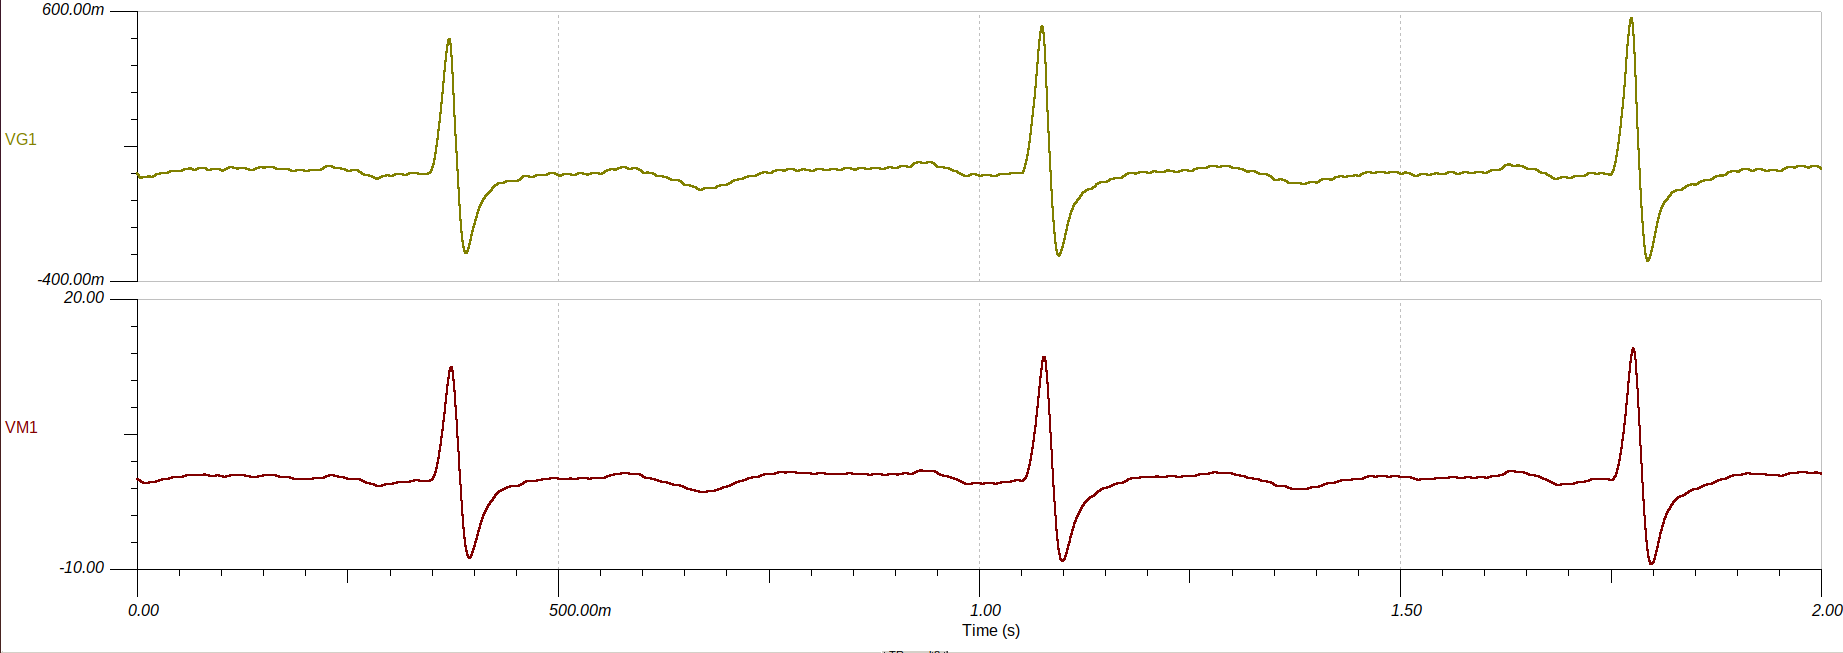
\includegraphics[width=0.9\textwidth]{final_ecg.png} 
  \caption{Circuit including Instrumentation Amplifier and Filter}
  \label{fig:instrumentation-amp}
\end{figure}

interestingly we can calculate the time period  of the heart beat which in this case is 0.7s which is close to the ideal value of 0.833s

\begin{figure}[h]
  \centering
  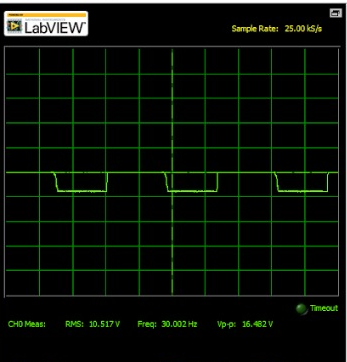
\includegraphics[width=0.5\textwidth]{scope.png} 
  \caption{Output Characteristics of output wave for sine wave of amplitude 0.025 V}
  \label{fig:instrumentation-amp}
\end{figure}


\end{document}
